\documentclass[11pt,a4paper, sans]{moderncv}

% Настройки пакетов
\usepackage[scale=0.85]{geometry}
\usepackage[T2A]{fontenc}
\usepackage[utf8]{inputenc}
\usepackage[english,russian]{babel}
\usepackage{xcolor}
\usepackage{enumitem}
\usepackage{fontawesome5}
\usepackage{graphicx}
\usepackage{cmap}
\usepackage{cmbright}
\usepackage{lettrine}

% Цветовая схема
\definecolor{primary}{RGB}{0, 100, 0} % тёмно-зелёный
\definecolor{secondary}{RGB}{34, 139, 34} % лесной зелёный
\definecolor{accent}{RGB}{50, 205, 50} % лаймовый

% Стиль CV
\moderncvstyle{banking}
\moderncvcolor{green}
\renewcommand{\familydefault}{\sfdefault}

% Настройка полей
\setlength{\hintscolumnwidth}{2.5cm}

% Кастомные команды
\newcommand{\cvproject}[4]{
    \cvitem{#1}{\textbf{#2}\hfill\href{#3}{\color{secondary}\faLink}\\
    \begin{minipage}[t]{\linewidth}\small\color{gray}#4\end{minipage}}
}

%===================================================================================================
% Основная информация
%===================================================================================================

\name{Куртеев}{Александр}
\title{Студент 2 курса ФРКТ МФТИ}
\address{Москва, Россия}
\phone[mobile]{+7 (952) 400-66-39}
\email{kurteev.am@phystech.edu}
\social[github]{HaipoviyPodrostok}
\social[telegram]{@Ryan\_gosling123456}

\begin{document}

\begin{minipage}{0.2\textwidth}
    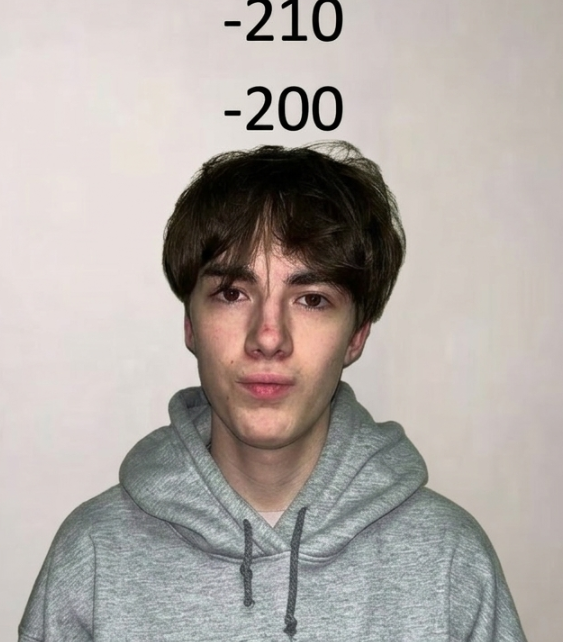
\includegraphics[width=90pt]{portret.png}
\end{minipage}% 
\begin{minipage}{0.8\textwidth}
    \makecvtitle
\end{minipage}

\section{\color{primary}\faGraduationCap\ Образование}
\cventry{2024--н.в.}{Бакалавриат}{МФТИ (ФРКТ)}{}{}{
\begin{itemize}[leftmargin=*,nosep]
    \item Прикладная математика и физика
\end{itemize}}

\section{\color{primary}\faCode\ Проекты}
\cvproject{Ноябрь 2026}{Графическая библиотека для пересечения треугольников}{https://github.com/HaipoviyPodrostok/Triangles}{
Реализация графической библиотеки для ускорения поиска пересечений лучей с треугольниками на C++. Реализация алгоритма LBVH с применением кодов Мортона. Поддержка гетерогенных вычислений: многопоточность на CPU и аппаратное ускорение на GPU посредством OpenCL.}

\cvproject{Сентябрь 2026}{Алгоритм кэширования 2Q}{https://github.com/HaipoviyPodrostok/Cache}{
Реализация алгоритма 2Q кэша на языке C++. Разработка эталонной модели (Ideal Cache) для сравнительного анализа эффективности алгоритмов на основе метрики попаданий (cache hits). Организация системы сборки через CMake и автоматизированного тестирования с использованием CTest.}

\cvproject{Февраль 2025}{Игра "Акинатор"}{https://github.com/HaipoviyPodrostok/Akinator}{
Консольная реализация игры "Акинатор" на языке C, в которой программа пытается угадать задуманного вами персонажа или предмет, задавая вопросы, на которые можно ответить "да" или "нет". Проект использует Бинарное дерево для хранения базы знаний. Обучение (добавление новых персонажей) происходит прямо во время игры.}

\cvproject{Декабрь 2026}{Прототип очков дополненной реальности}{https://github.com/HaipoviyPodrostok/Prompter-glasses}{
Рабочий функциональный прототип очков дополненной реальности. В данной реализации используются как очки-телесуфлеры. Очки-суфлёры — устройство, которое позволяет читать заготовленный текст. Текст проецируется на полупрозрачное зеркало и становится доступным для прочтения только для пользователя. Это решает проблему мобильности студийных телесуфлеров.}

\section{\color{primary}\faCogs\ Навыки}
\begin{itemize}[leftmargin=*,nosep]
    \item \textbf{Языки программирования}: C/C++, OpenCL, \LaTeX.
    \item \textbf{Инструменты}: Git, Linux, Make/CMake, matplotlib, HTML/CSS, GDB.
    \item \textbf{Инженерия}: Fusion 360, SolidWorks, черчение, работа с лазерным станком, 3D-принтером, пайка, обработка материалов.
    \item \textbf{Языки}: Английский (B2), Русский (родной).
\end{itemize}

\end{document}